
% Title page.
\title[Aula 02]{Ondas e Marés}
\subtitle{Introdução}
\author[Filipe Fernandes]{Filipe P. A. Fernandes}
\institute[unimonte]{Centro Universitário Monte Serrat}
\date[Agosto 2013]{16 de Agosto 2013}

\logo{\includegraphics[scale=0.15]{../common/university_logo.png}}

\begin{document}

% The title page frame.
\begin{frame}[plain]
  \titlepage
  \begin{center}
    \includegraphics[scale=0.5]{../common/by-nc-sa.pdf}
  \end{center}
\end{frame}

\section*{Outline}
\begin{frame}
\tableofcontents
\end{frame}

\section{{Introdução: O que são ondas?}}

\begin{frame}
\frametitle{Introdução: O que são ondas?}
    \begin{block}{}
      Ondas são deformações periódicas em uma interface.  Em oceanografia, ondas
      de superfície são deformações da superfície dos oceanos, i.e., na
      interface oceano-atmosfera.
    \end{block}
\end{frame}


\begin{frame}
  \frametitle{Introdução: O que são ondas?}
  \begin{block}{}
    As deformações se propagam com a velocidade de onda,
    enquanto as partículas descrevem movimentos oscilatórios ou orbitais com
    velocidade de partículas e permanecem, em média, na mesma posição.
  \end{block}
\end{frame}


\begin{frame}
\frametitle{Introdução: O que são ondas?}
    \begin{block}{}
      Em águas profundas, os caminhos das partículas são circulares.
    \end{block}

    \begin{block}{}
      Em águas mais rasas, os caminhos percorridos pelas partículas se achatam e
      ficam parecendo elipses.
    \end{block}
\end{frame}


\begin{frame}
\frametitle{Introdução: O que são ondas?}
  \begin{block}{}
    Uma onda de águas profundas passa a ser considerada
    como de águas rasas quando o comprimento de onda $\lambda$ se torna maior
    do que o dobro da profundidade local da água $h$.
  \end{block}

  \begin{block}{}
    As mudanças nas propriedades das ondas entretanto ocorrem antes disso,
    quando $\lambda = 20 h$.
  \end{block}
\end{frame}


\begin{frame}
\frametitle{Teoria linear de ondas de gravidade livres}
\scriptsize{
    \begin{block}{{\bf Não forçado}}
        Considera o movimento oscilatório (ondulatório) apenas a partir do
        momento em que a forçante que causou o movimento já não existe mais
    \end{block}

    \pause
    \begin{block}{{\bf Sem atrito}}
        O período das mesmas é bem menor que o período necessário para que o
        efeito de atenuação causado pelo atrito interno do fluido seja
        considerável.
    \end{block}

    \pause
    \begin{block}{{\bf Sem influência da terra.}}
        Ondas de gravidade tem um período muito curto quando comparado ao
        período inercial, e portanto os efeitos de rotação da Terra podem ser
        negligenciados.
    \end{block}
}
\end{frame}

\begin{frame}
  \frametitle{``I think you should be more explicit here in step two...''}
  \includegraphics[scale=0.45]{./figures/then-a-miracle-occurs-cartoon.png}
  % Copyright © 2013 by Sidney Harris.
  % No reproduction other than for personal enjoyment without written permission.
\end{frame}

\section{Definições}
\begin{frame}
  \frametitle{Definições (Resposta do exercício 00)}
  \begin{center}
    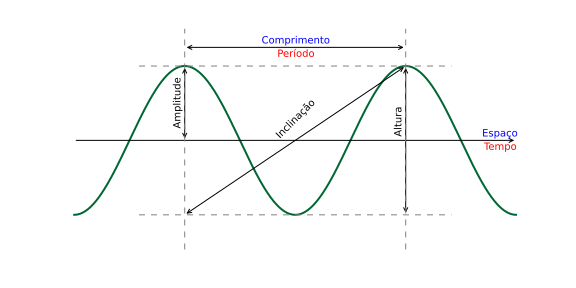
\includegraphics[scale=0.7]{../Aula_01/figures/wave_definitions.pdf}
  \end{center}
\end{frame}

\begin{frame}
\frametitle{Descrição das Ondas}
  \begin{block}{}
    A maneira mais simples de encarar as ondas é pelo conceito da onda como uma
    oscilação harmônica. Assim, podemos descrevê-las por
  \end{block}
    \begin{itemize}[<+-| alert@+>]
      \item período T
      \item frequência $\omega = 2 \pi / \text{T}$
      \item comprimento de onda $\lambda$
      \item velocidade $c = \lambda / \text{T}$
      \item altura H = 2 A (A = amplitude)
      \item inclinação $\delta = \text{H} / \lambda$
    \end{itemize}
\end{frame}

\begin{frame}
\frametitle{Ondas longas vs ondas curtas}
  \small{
  \begin{block}{}
  \begin{center}
    $0 < \underbrace{\lambda}_{\substack{\text{água profunda} \\\text{ondas curtas}}}
    < 2 \text{h} < \underbrace{\lambda}_{\substack{\text{ondas de} \\\text{transição}}}
    < 20 \text{h} < \underbrace{\lambda}_{\substack{\text{água rasa} \\\text{ondas longas}}}$
  \end{center}
  \end{block}
}
\end{frame}

\begin{frame}
\frametitle{Ondas de água profundas (ondas curtas)}
    \begin{center}
        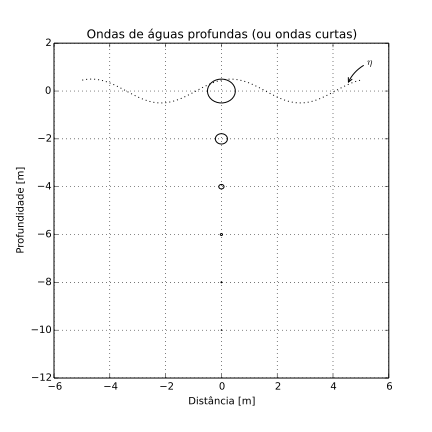
\includegraphics[scale=0.7]{./figures/deep_water_waves.pdf}
    \end{center}
\end{frame}

\begin{frame}
\frametitle{Ondas longas vs ondas curtas}
    \begin{center}
        \includegraphics[scale=0.45]{./figures/deep_to_shallow.png}
    \end{center}
\end{frame}

\begin{frame}
\frametitle{Ondas de água rasa (ondas longas)}
    \begin{center}
        \includegraphics[scale=0.7]{./figures/shallow_water_waves.pdf}
    \end{center}
\end{frame}


\section{Velocidades de fase e grupo}
\begin{frame}
\frametitle{Superposição de ondas}
    \begin{block}{}
        A superposição de duas ondas com frequências bem próximas $\omega_1$ e
        $\omega_2$ respectivamente, produz grupos de ondas ou séries.
    \end{block}

    \pause
    \begin{block}{}
        As cristas individuais propagam com uma velocidade de fase (ou
        velocidade da onda) $c$;  séries de ondas propagam com uma velocidade
        de grupo:
    \end{block}
\end{frame}

\begin{frame}
\frametitle{Superposição de ondas}
    \begin{block}{}
        \begin{center}
            \[
                c_g = c - \lambda \frac{dc}{d\lambda} \text{ ou,}
            \]
            \[
                c_g = \frac{d\omega}{d\kappa}
            \]
        \end{center}
    \end{block}
\end{frame}

\begin{frame}
\frametitle{Dever de casa 01}
    \begin{block}{}
        Usando a equação do exercício anterior produza 5 gráficos:
        \begin{itemize}
            \item $x = 0$, onda fixa num ponto no espaço;
            \item $t = 0$, uma "fotografia de uma onda".  Faça essa onda
                  coincidir com a anterior;
            \item Escolha um dos gráficos acima e varie a sua fase para:
                  90\textdegree{}, 180\textdegree{}, e 270\textdegree{}.
        \end{itemize}
    \end{block}
\end{frame}

\begin{frame}
\frametitle{Aula de reposição...}
    \begin{block}{}
        Não teremos aula nos dias 23 e 30 de Agosto.
    \end{block}
\end{frame}

\end{document}
